%% chapter 4 dataset, network structure, experiment and result
\chapter{实验结果}
\section{掌静脉数据集}
本文选用香港理工大学静脉图像库
\footnote{数据来源URL:\url{https://gitcode.com/open-source-toolkit/beb78}},该数据库提供的是香港理工大学多光谱图像库中的近红外光手掌图像库,即掌静脉图像库。
包含了500名参与者的掌静脉图像,适用于生物识别、图像处理等领域的研究和应用。读取数据集,部分图片参见\autoref{fig:palmvein1};与掌纹图像的对比参见\autoref{fig:multi-image-example1}
\begin{figure}[!htbp]
    \centering
    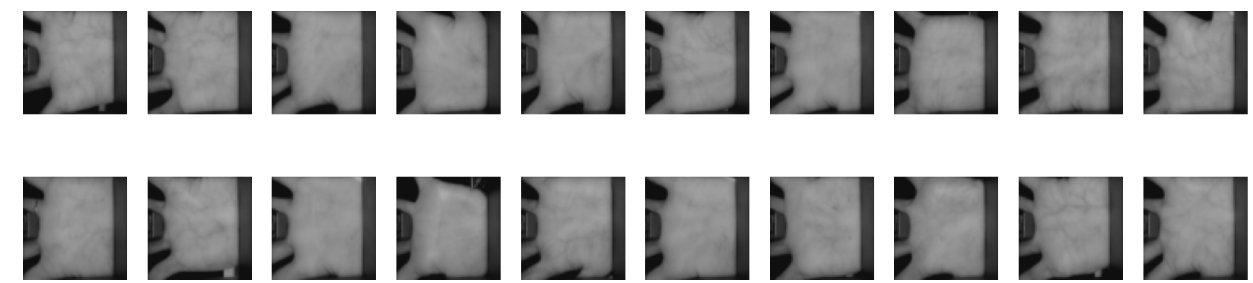
\includegraphics[scale = 0.6]{image/chap04/palmvein1.png}
    \caption{掌静脉图像}
    \label{fig:palmvein1}
\end{figure}

\begin{figure}[h!]
    \centering
    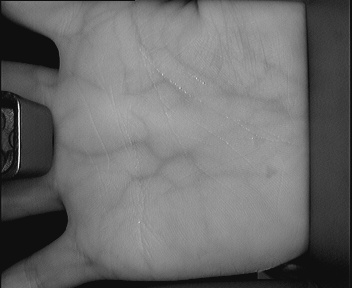
\includegraphics[width=.16\textwidth,height=.12\textwidth]{image/chap04/1_01.jpg}
    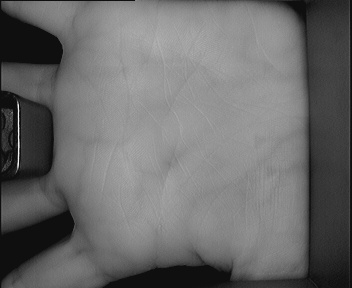
\includegraphics[width=.16\textwidth,height=.12\textwidth]{image/chap04/1_03.jpg}
    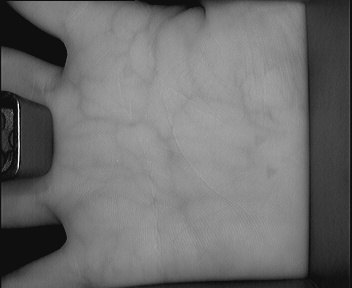
\includegraphics[width=.16\textwidth,height=.12\textwidth]{image/chap04/1_04.jpg}
    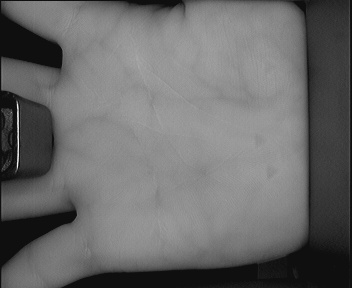
\includegraphics[width=.16\textwidth,height=.12\textwidth]{image/chap04/2_05.jpg}
    \\
    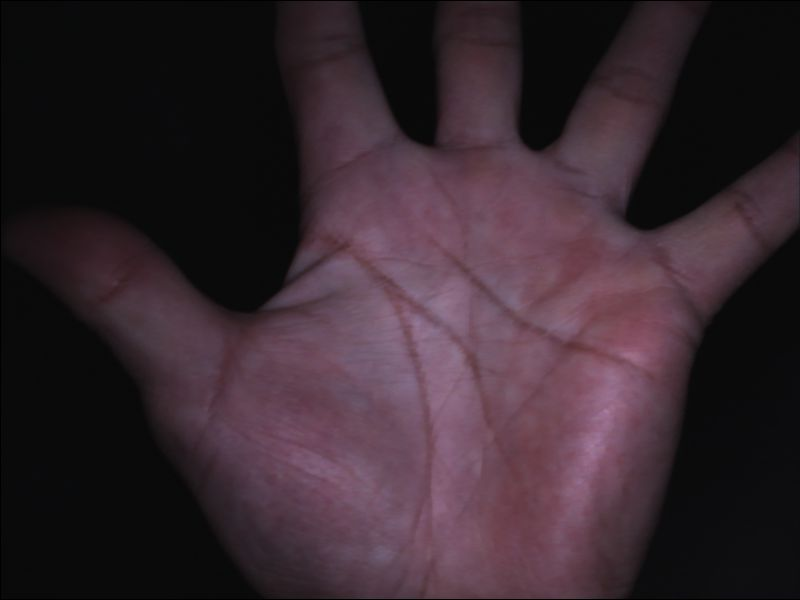
\includegraphics[width=.16\textwidth,height=.12\textwidth]{image/chap04/00003.jpg}
    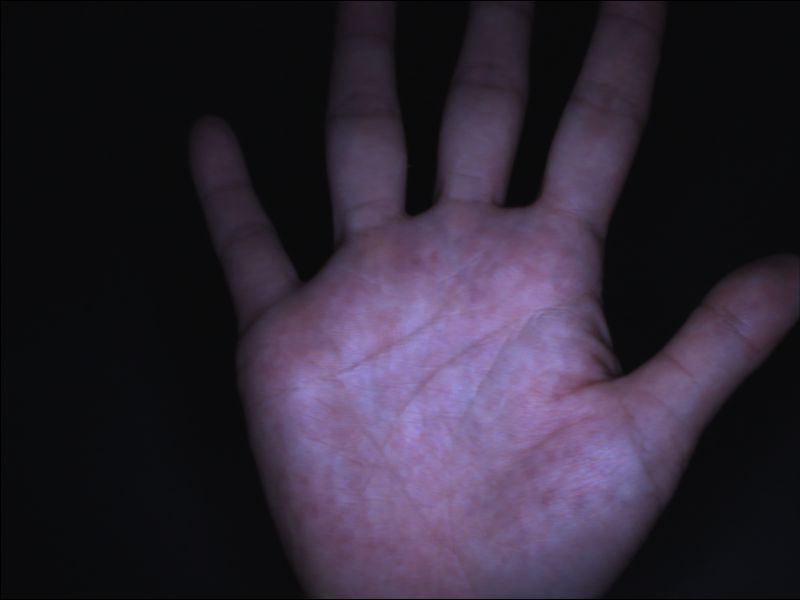
\includegraphics[width=.16\textwidth,height=.12\textwidth]{image/chap04/00079.jpg}
    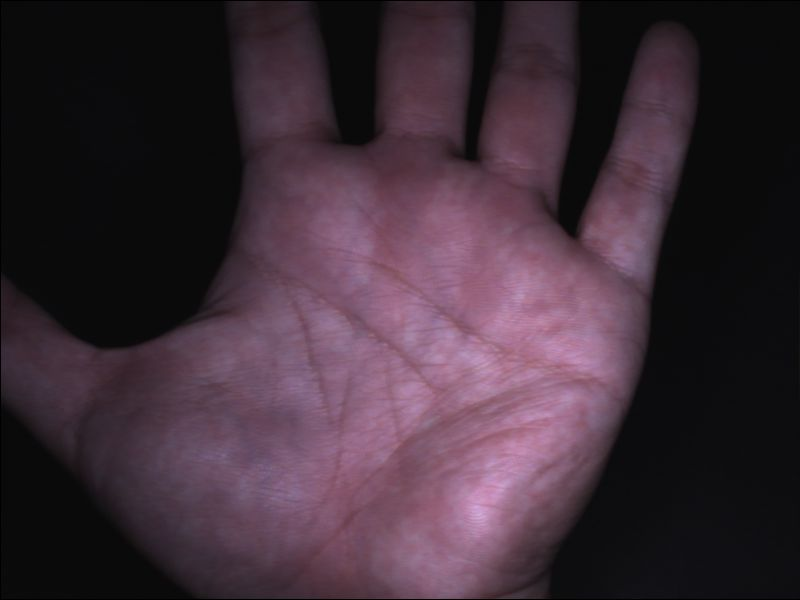
\includegraphics[width=.16\textwidth,height=.12\textwidth]{image/chap04/00142.jpg}
    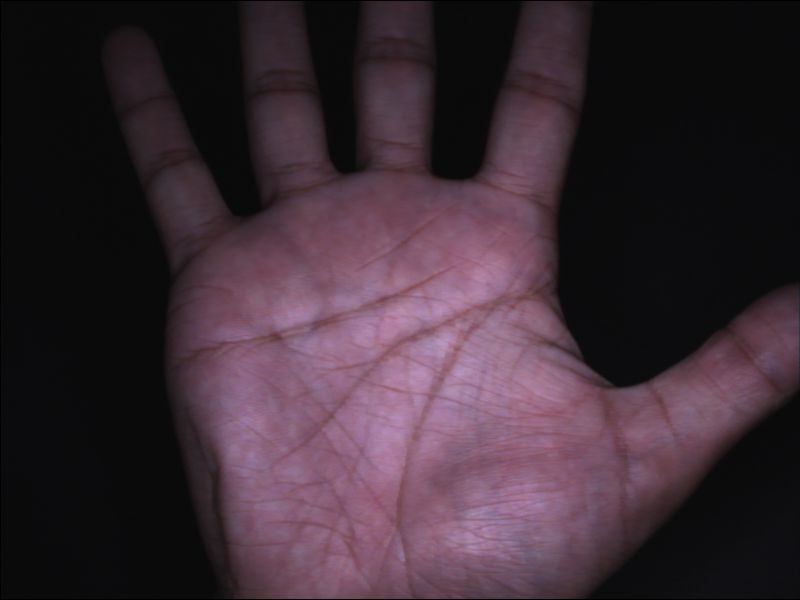
\includegraphics[width=.16\textwidth,height=.12\textwidth]{image/chap04/00175.jpg}
    \caption{掌静脉图像与掌纹图像对比}
    \label{fig:multi-image-example1}
\end{figure}

掌静脉图像的原始图像尺寸过大且对比度不够,掌静脉纹理信息在显示上并不清楚。
本文对原始图像做预处理,包括对比度调整,尺寸调整为64x64或32x32分辨率大小,便于个人计算机的小参数量深度神经网络的训练。

\begin{figure}[!htbp]
    \centering
    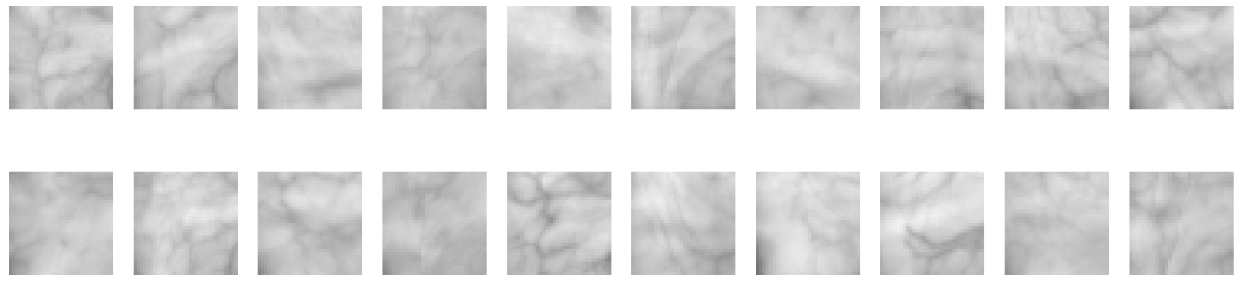
\includegraphics[scale = 0.5]{image/chap04/palmvein2.png}
    \caption{掌静脉局部图像(用于实验)}
    \label{fig:palmvein2}
\end{figure}

\section{对抗生成网络实验结果}
对64x64的掌静脉图像训练,应用改进技术:标签平滑化、特征匹配技术。下图给出了生成器与判别器的损失随训练过程进行的改变
\begin{figure}[!htbp]
    \centering
    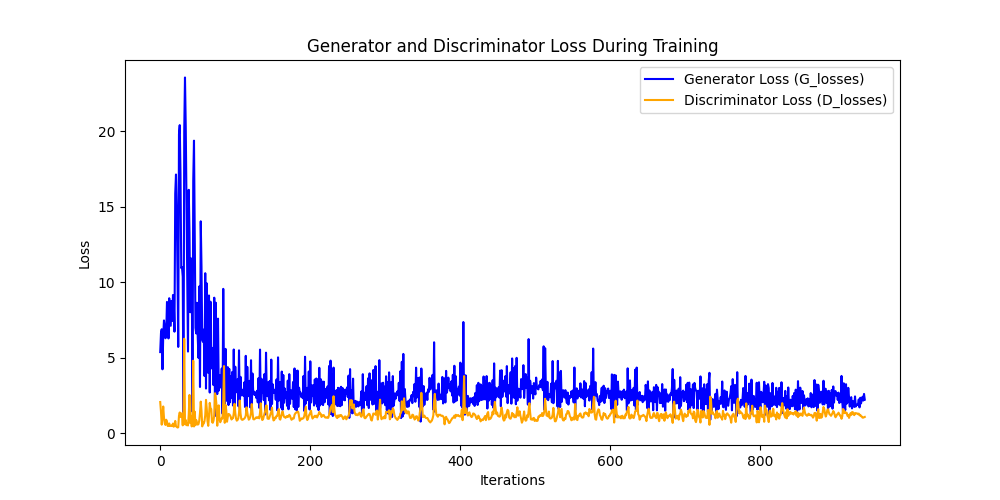
\includegraphics[scale = 0.5]{image/chap04/GAN/loss.png}
    \caption{DCGAN损失曲线}
    \label{fig:DCGAN_loss}
\end{figure}

经过20epochs后的DCGAN训练结果
\begin{figure}[!htbp]
    \centering
    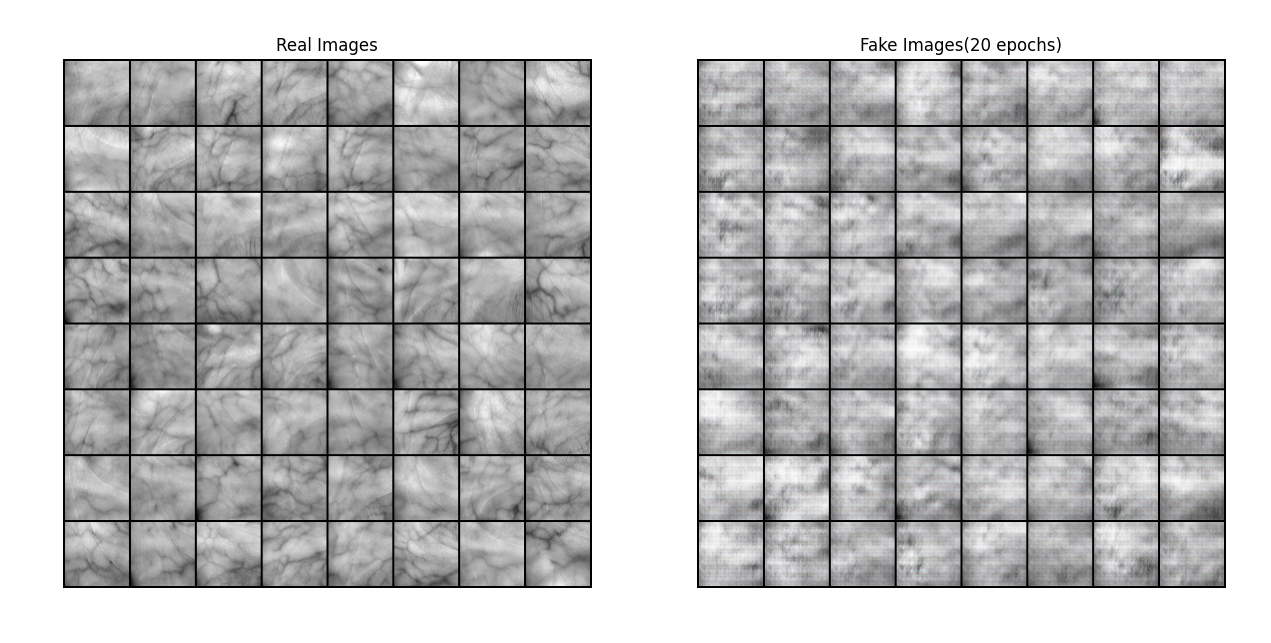
\includegraphics[width=15cm]{image/chap04/GAN/DCGAN_image.png}
    \caption{DCGAN生成图片与真实图片对比}
    \label{fig:DCGAN_img}
\end{figure}
生成图片在掌静脉纹理已经有不错的生成效果,然而生成图片仍然存在一定的棋盘状伪影(反卷积层产生的间隙导致上采样结果不够平滑),这预示着DCGAN的训练依然不够充分。

\section{扩散模型实验结果}
\begin{figure}[!htbp]
    \centering
    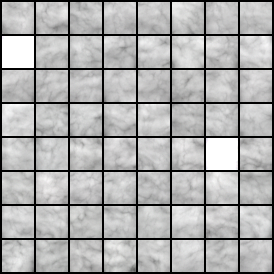
\includegraphics[width=10cm]{image/chap04/Diffusion/linearnoise_image.png}
    \caption{扩散模型生成结果}
    \label{fig:DCGAN_img}
\end{figure}
